\documentclass[a4paper,11pt]{article}

\usepackage[T1]{fontenc}

% \usepackage[light,math]{iwona}

%\usepackage[light]{iwona} % keep math in old-school font

\usepackage[utf8]{inputenc}

\usepackage{lmodern}

\usepackage{float}

\usepackage{pdfpages}

\usepackage[dvipsnames]{xcolor}

\usepackage[finnish, british]{babel}

\usepackage{amsmath}

\usepackage[affil-it]{authblk}          % to enable \affil

\usepackage{cancel}

\usepackage{hyperref}               % to enable \texorpdfstring

\usepackage{cleveref}

\usepackage{graphicx}

\usepackage{natbib}             %for citations in Harvard style

\usepackage{enumerate}          %to be able to change the enumerate symbols

\usepackage{amsfonts}           % for special set symbols

\usepackage{listings}

\usepackage{cleveref}

\usepackage{a4wide}

\usepackage{fancyhdr}

\setlength{\headheight}{26pt}

\usepackage{mathrsfs}

\pagestyle{fancy}

\newcommand{\crefrangeconjunction}{--}

\lstset{
        language=Matlab,
        breaklines=true
    }

\lhead{Homework 3\\ October 19, 2026}

\chead{Computational Physics}

\rhead{Jasmine Palma Gomez\\ PHYS-GA 2000}

\renewcommand{\headrulewidth}{0.4pt}

\DeclareMathOperator*{\argmin}{arg\,min}

\DeclareMathOperator*{\argmax}{argmax}

\DeclareMathOperator*{\var}{Var}

\newcommand{\E}{\mathbb{E}}

\graphicspath{{./plotit/}}


\makeatother                            % restores '@' to its normal function

%\renewcommand{\thesection}{\Alph{section}}

%\renewcommand{\thesubsection}{\arabic{subsection}}

%\renewcommand{\thesubsubsection}{\alph{subsubsection}}

\begin{document}

\section*{Summary}

In this assignment, we explore the use of Fourier transforms to analyze periodic signals, smooth data by filtering high frequency noise, and reconstruct a blurred image via deconvolution. The sunspot data showed a dominant Fourier peak corresponding to a period of approximately 11 years, which agrees well with the known solar cycle. For the Dow Jones dara, retaining only the lowest frequency Fourier coefficients produced progressively smoother approximations by discarding high frequency noise to capture the underlying broad trend. Finally, by constructing a periodic Gaussian point spread function and making use of the convolution theorem in Fourier space, we were able to deconvolve a blurred image of a house and recover a clearer representation of the original image by dividing the Fourier transform of the blurred image by that of the point spread function, followed by an inverse Fourier transform to return to real space. The reconstruction improved the image, although it was not perfecr because very small Fourier components of the point spread function cannot be safely divided without amplifying numerical errors and noise. 


\section*{Methods}

\subsection*{Exercise 7.2: Detecting Periodicity}

\subsubsection*{Time Series Data and Initial Estimate}

The observed number of sunspots since Januart 1749 was read from the file \texttt{sunspots.txt} and plotted as a function of month. The period of the solar cycle was first estimated directly from the data by identifying groups of months with less than 10 sunspot counts. Consecutive low sunspot months were grouped into separate solar minima, and the average separation between these minima was used as an initial estimate of the cycle length.

\subsubsection*{Fourier Power Spectrum}

To identify periodic components more precisely, the discrete Fourier transform of the sunspot signal was calculated. For a signal containing $N$ samples, the Fourier coefficients are
\[ c_k = \sum_{n=0}^{N-1} s_n \exp\left(-\frac{2\pi i kn}{N}\right),\] where $s_n$ is the sunspot number at month $n$. The power spectrum was then computed as \[P_k = |c_k|^2.\]

Because the sunspot signal contains only real values, its Fourier spectrum is symmetric, so the second half contains duplicate negative frequency information and only the first \(N//2+1\) coefficients are unique. Therefore, we only keep the first half of the power spectrum.

\subsubsection*{Frequency and Period}

The dominant nonzero peak in the power spectrum determines the principal periodic component of the signal. Since the data are sampled once per month, the frequency corresponding to index $k$ is
\[f_k = \frac{k}{N} \, \text{cycles per month}. \] The corresponding period is \[T_k = \frac{1}{f_k} = \frac{N}{k} \, \text{months}.\]
The period associated with the largest nonzero power was compared with the cycle length estimated directly from the solar minimum data.

\subsection*{Exercise 7.4: Fourier Filtering and Smoothing}

\subsubsection*{Fourier Representation of the Data}

The daily Dow Jones closing values from late 2006 to the end of 2010 were read from \texttt{dow.txt} and plotted as a function of trading day. The discrete Fourier coefficients were calculated using the real fast Fourier transform, \texttt{rfft}, which returns the independent nonnegative frequency coefficients of the real valued time series.

\subsubsection*{Low Frequency Filtering}

To construct a smoothed approximation, all but the first $10\%$ of the Fourier coefficients were set equal to zero. The filtered signal was then reconstructed using the inverse real Fourier transform, \texttt{irfft}. Retaining only the lowest frequency coefficients preserves the slowly varying behavior of the stock market data while removing many of its short term fluctuations. This is useful because we are mainly interested in the broad trend of the data rather than noisy day-to-day variations.

\subsubsection*{Comparison of Different Resolutions}

The filtering procedure was repeated while retaining only the first $2\%$ of the Fourier coefficients. The resulting signals were compared with the original data and with the $10\%$ reconstruction. Retaining fewer Fourier coefficients produces a smoother curve because more of the higher frequency components responsible for the short term fluctuations have been removed, distilling the essential features of the data even more than the $10\%$ case.

\subsection*{Exercise 7.9: Image Deconvolution}

\subsubsection*{Image Blurring as a Convolution}
The blurred image was read from \texttt{blur.txt} and represented as a two dimensional array $b(x,y)$. Following the textbook, the blurred image is modeled as the convolution of an unblurred image $a(x,y)$ with a point spread function $f(x,y)$:
\[b(x,y) = \int_0^K\int_0^L a(x',y')f(x-x',y-y')\,dx'\,dy'.\]
The point spread function describes how the brightness of an individual point is distributed over neighboring pixels.

\subsubsection*{Periodic Gaussian Point Spread Function}

The point spread function was modeled as a Gaussian with width
$\sigma=25$: \[f(x,y) = \exp\left[ -\frac{x^2+y^2}{2\sigma^2}\right].\]
Because the Fourier transform assumes periodic boundary conditions, the coordinates were defined periodically. To explicitly implement this, the $x$ and $y$ coordinates were shifted so that the origin is at the center of the arrsay in the following manner:
\[x \leftarrow \begin{cases} x, & x \leq N_x/2,\\ x-N_x, & x>N_x/2, \end{cases} \qquad y \leftarrow \begin{cases} y, & y \leq N_y/2,\\ y-N_y, & y>N_y/2. \end{cases}\]
Thus, indices near the end of the array represent negative coordinates near the origin. This produces the bright patches in all four corners of the point spread function array.

\subsubsection*{Fourier-Space Deconvolution}

The blurred image is simply the convolution of the original image with the point spread function. The convolution theorem thus states that the Fourier transform of the blurred image is related to the transforms of the original image and point spread function by
\[\widetilde{b}_{kl} = KL\,\widetilde{a}_{kl}\widetilde{f}_{kl},\] where $K\times L$ is the image size. Therefore, the Fourier coefficients of the unblurred image can be obtained by dividing by the Fourier transform of the point spread function:
\[\widetilde{a}_{kl} = \frac{\widetilde{b}_{kl}}{KL\,\widetilde{f}_{kl}}.\]
The two-dimensional real fast Fourier transform, \texttt{rfft2}, was applied to both the blurred image and the point spread function, and the result was converted back to pixel space using \texttt{irfft2}. In the numerical implementation, Fourier coefficients satisfying $|\widetilde{f}_{kl}|<10^{-3}$ were not divided by, instead their corresponding blurred-image coefficients were left unchanged. This avoids division by zero or by values so small that they would produce unstable results and amplify numerical errors. The resulting image was then displayed as the deconvolved reconstruction.

\section*{Results}

\subsection*{Exercise 7.2: Detecting Periodicity}

The sunspot data exhibits clear periodic behavior in time. The grouping of low sunspot months provides a good estimate of the average cycle length, with successive minima separated by roughly 132 months (11 years). (See \cref{fig:sunspot-minimums}.)

\begin{figure}[H]
    \centering
    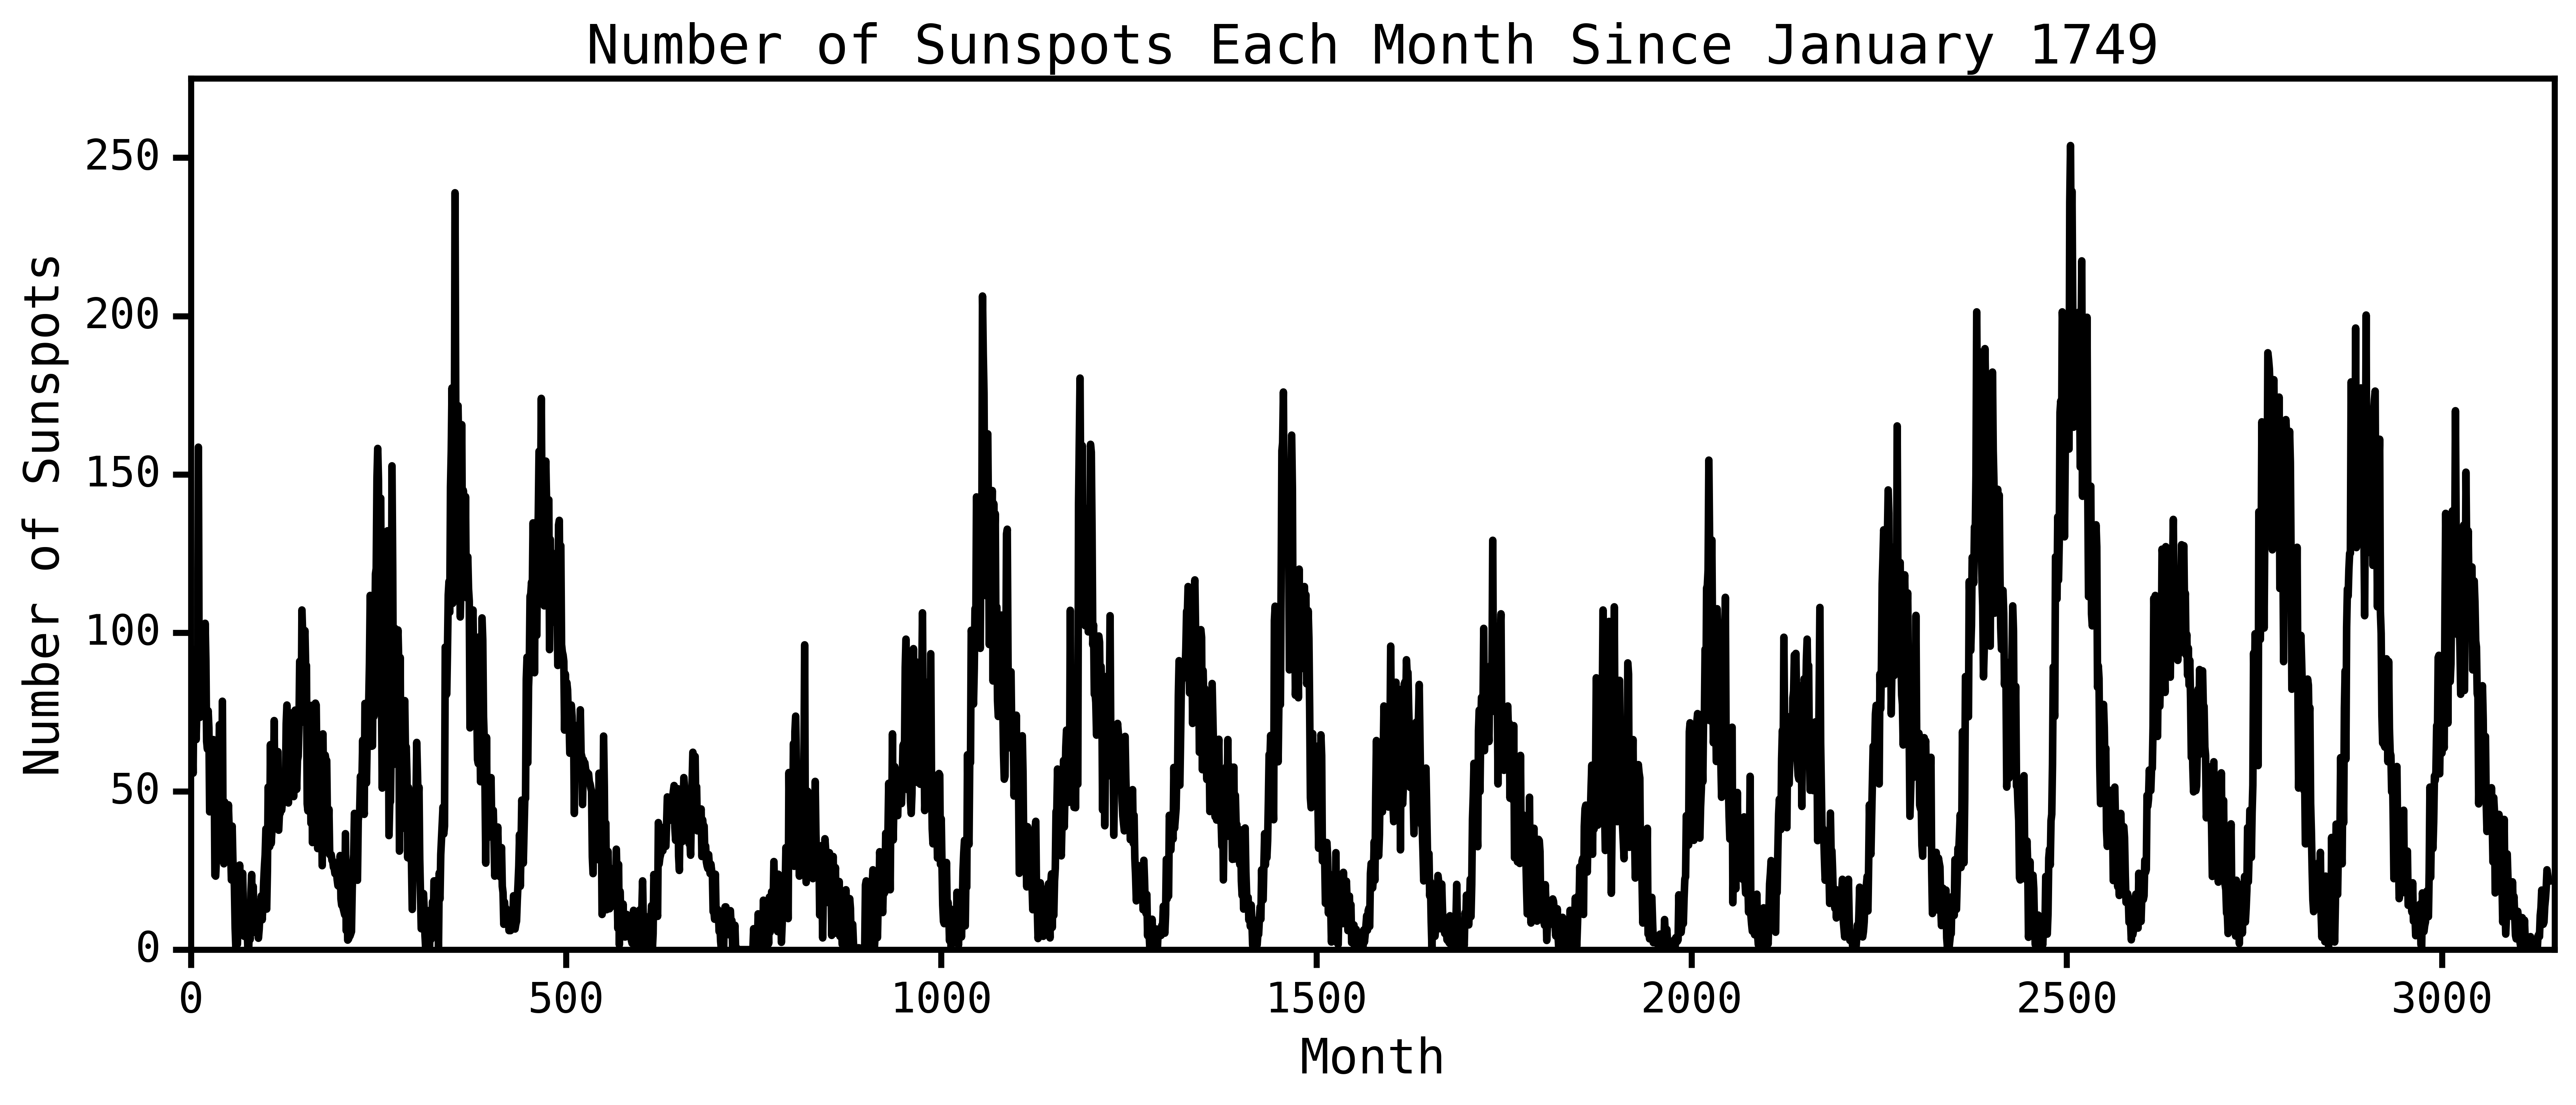
\includegraphics[width=0.95\textwidth]{figures/sunspots.png}
    \vspace{0.5em}
    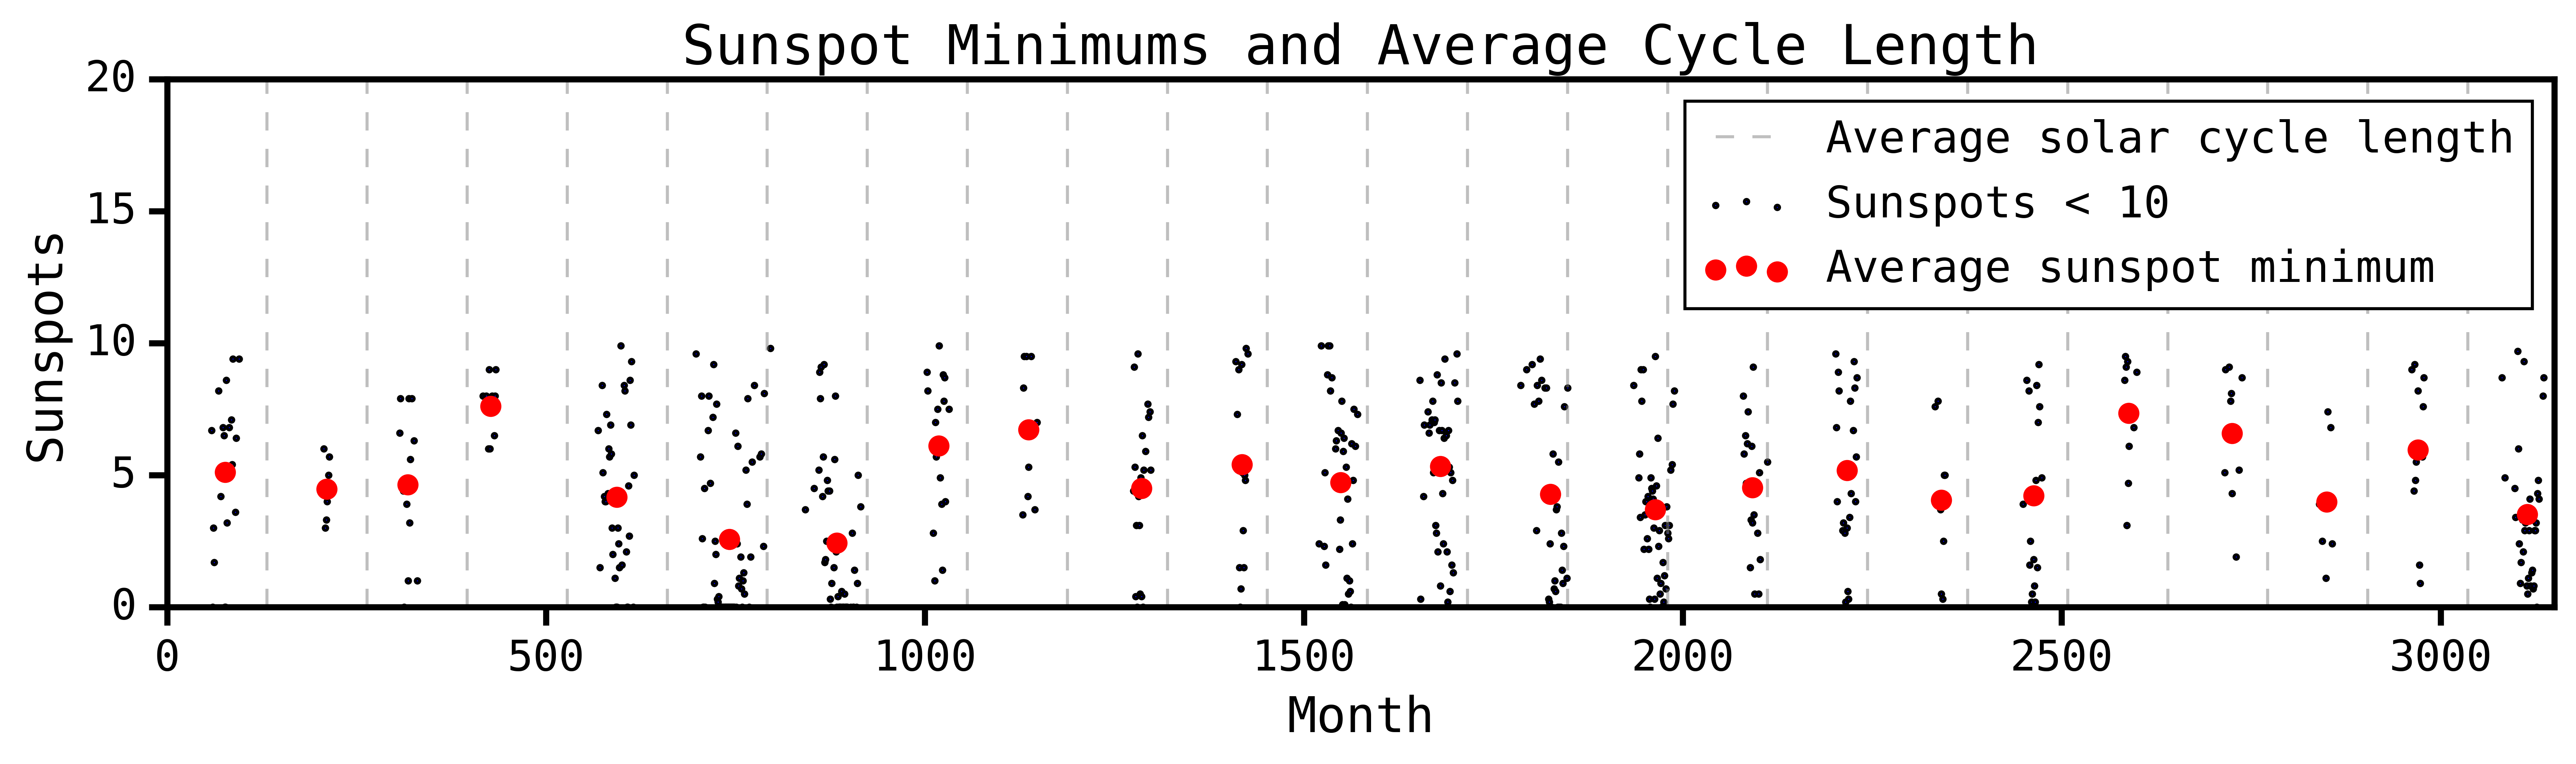
\includegraphics[width=0.95\textwidth]{figures/solar_minimums.png}
    \caption{Top: Monthly sunspot numbers from January 1749 onward. Bottom:
    Identified solar-minimum groups and the estimated average separation between successive minima to be 132 months (11 years).}
    \label{fig:sunspot-minimums}
\end{figure}

The Fourier power spectrum in \cref{fig:sunspot-power} gives a more precise frequency-domain description of the signal's periodicity.
\begin{figure}[H]
    \centering
    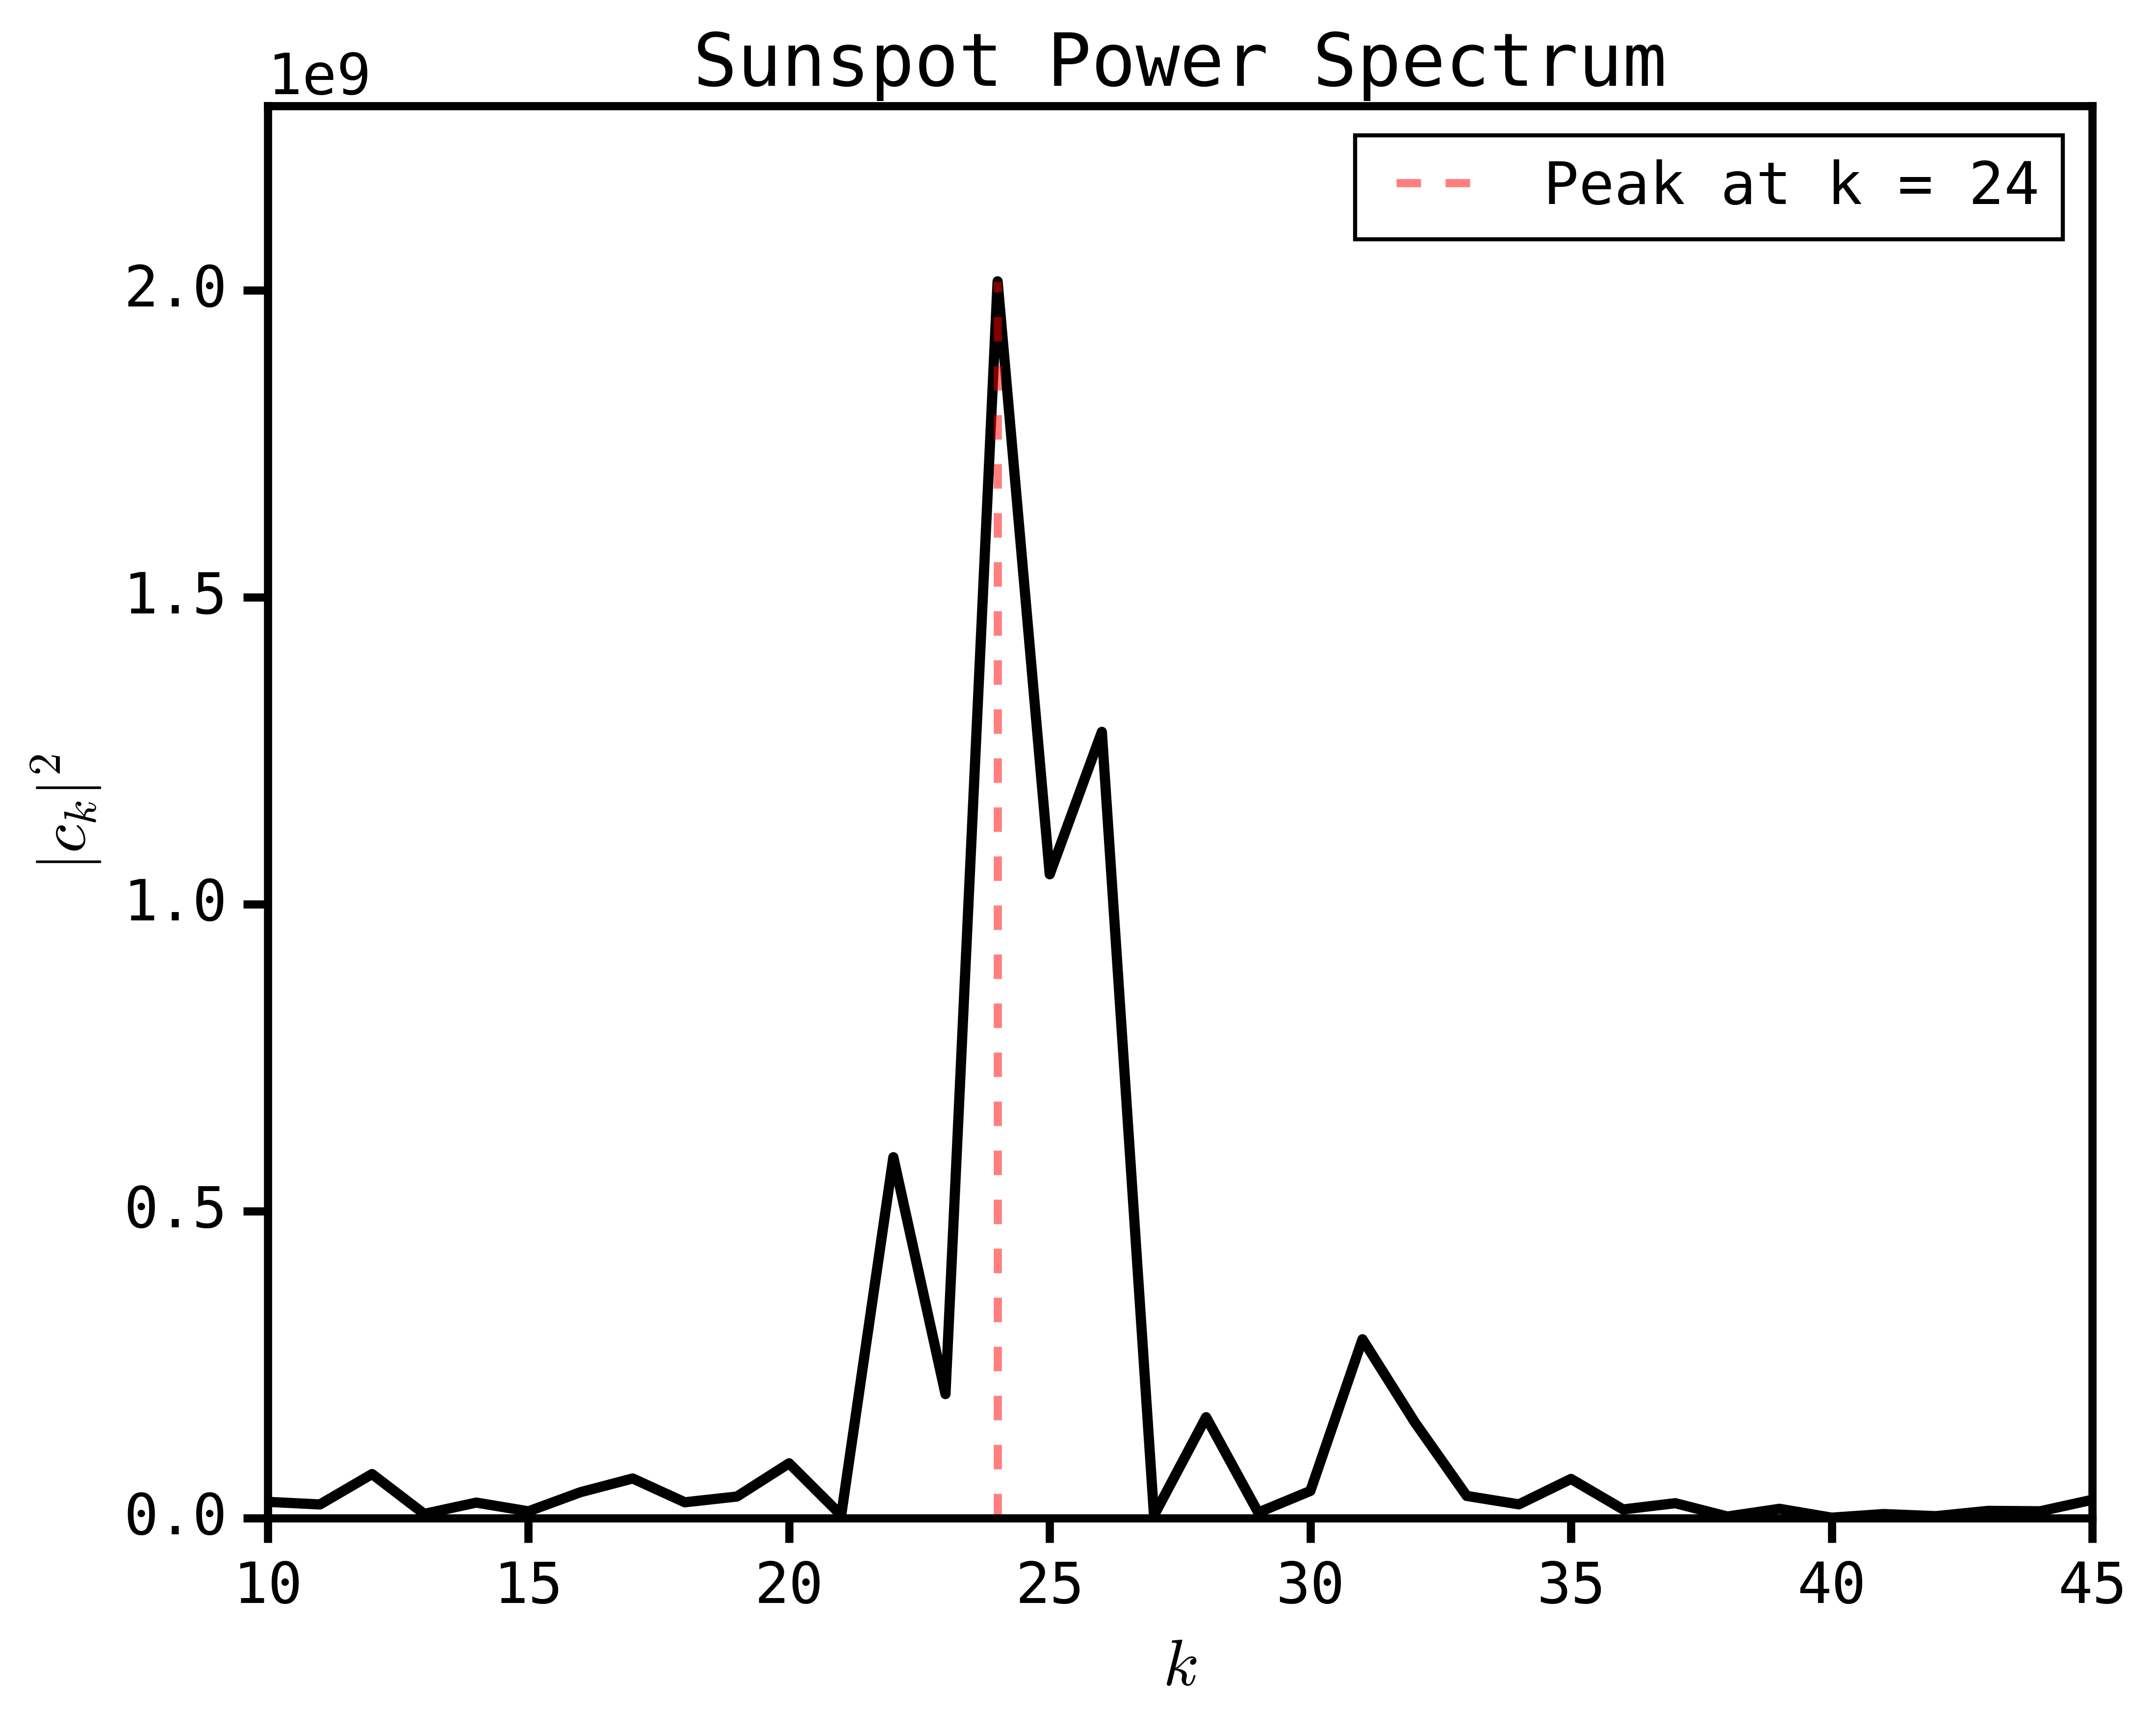
\includegraphics[width=0.75\textwidth]{figures/sunspot_power_spectrum.png}
    \caption{Power spectrum of the sunspot signal. The prominent nonzero peak identifies the dominant periodic component of the data, which is at wavenumber $k=24$.}
    \label{fig:sunspot-power}
\end{figure}

This peak in the power spectrum corresponds to the wavenumber $k=24$, which gives a frequency of $f_{24} = 0.0076$ cycles per month and a period of $T_{24} = 130.9584$ months, which is in good agreement with the initial estimate from the solar minimum data above. Even though the oscillation in our data isn't a perfect sine wave, the Fourier transform was still able to discern the dominant period of the signal.

\subsection*{Exercise 7.4: Fourier Filtering and Smoothing}

The original Dow Jones data has both slowly varying trends and quick fluctuations. Retaining only the first $10\%$ of the Fourier coefficients removes much of the high frequency variation while preserving the overall behavior of the signal. When only the first $2\%$ of the coefficients are kept, the reconstructed curve becomes even smoother and represents only the broadest trends in the data. Consequently, the low frequency Fourier coefficients describe long term variations, while the high frequency coefficients describe fine details, noise, and short lived fluctuations. (See \cref{fig:dow-filtering}.)

\begin{figure}[H]
    \centering
    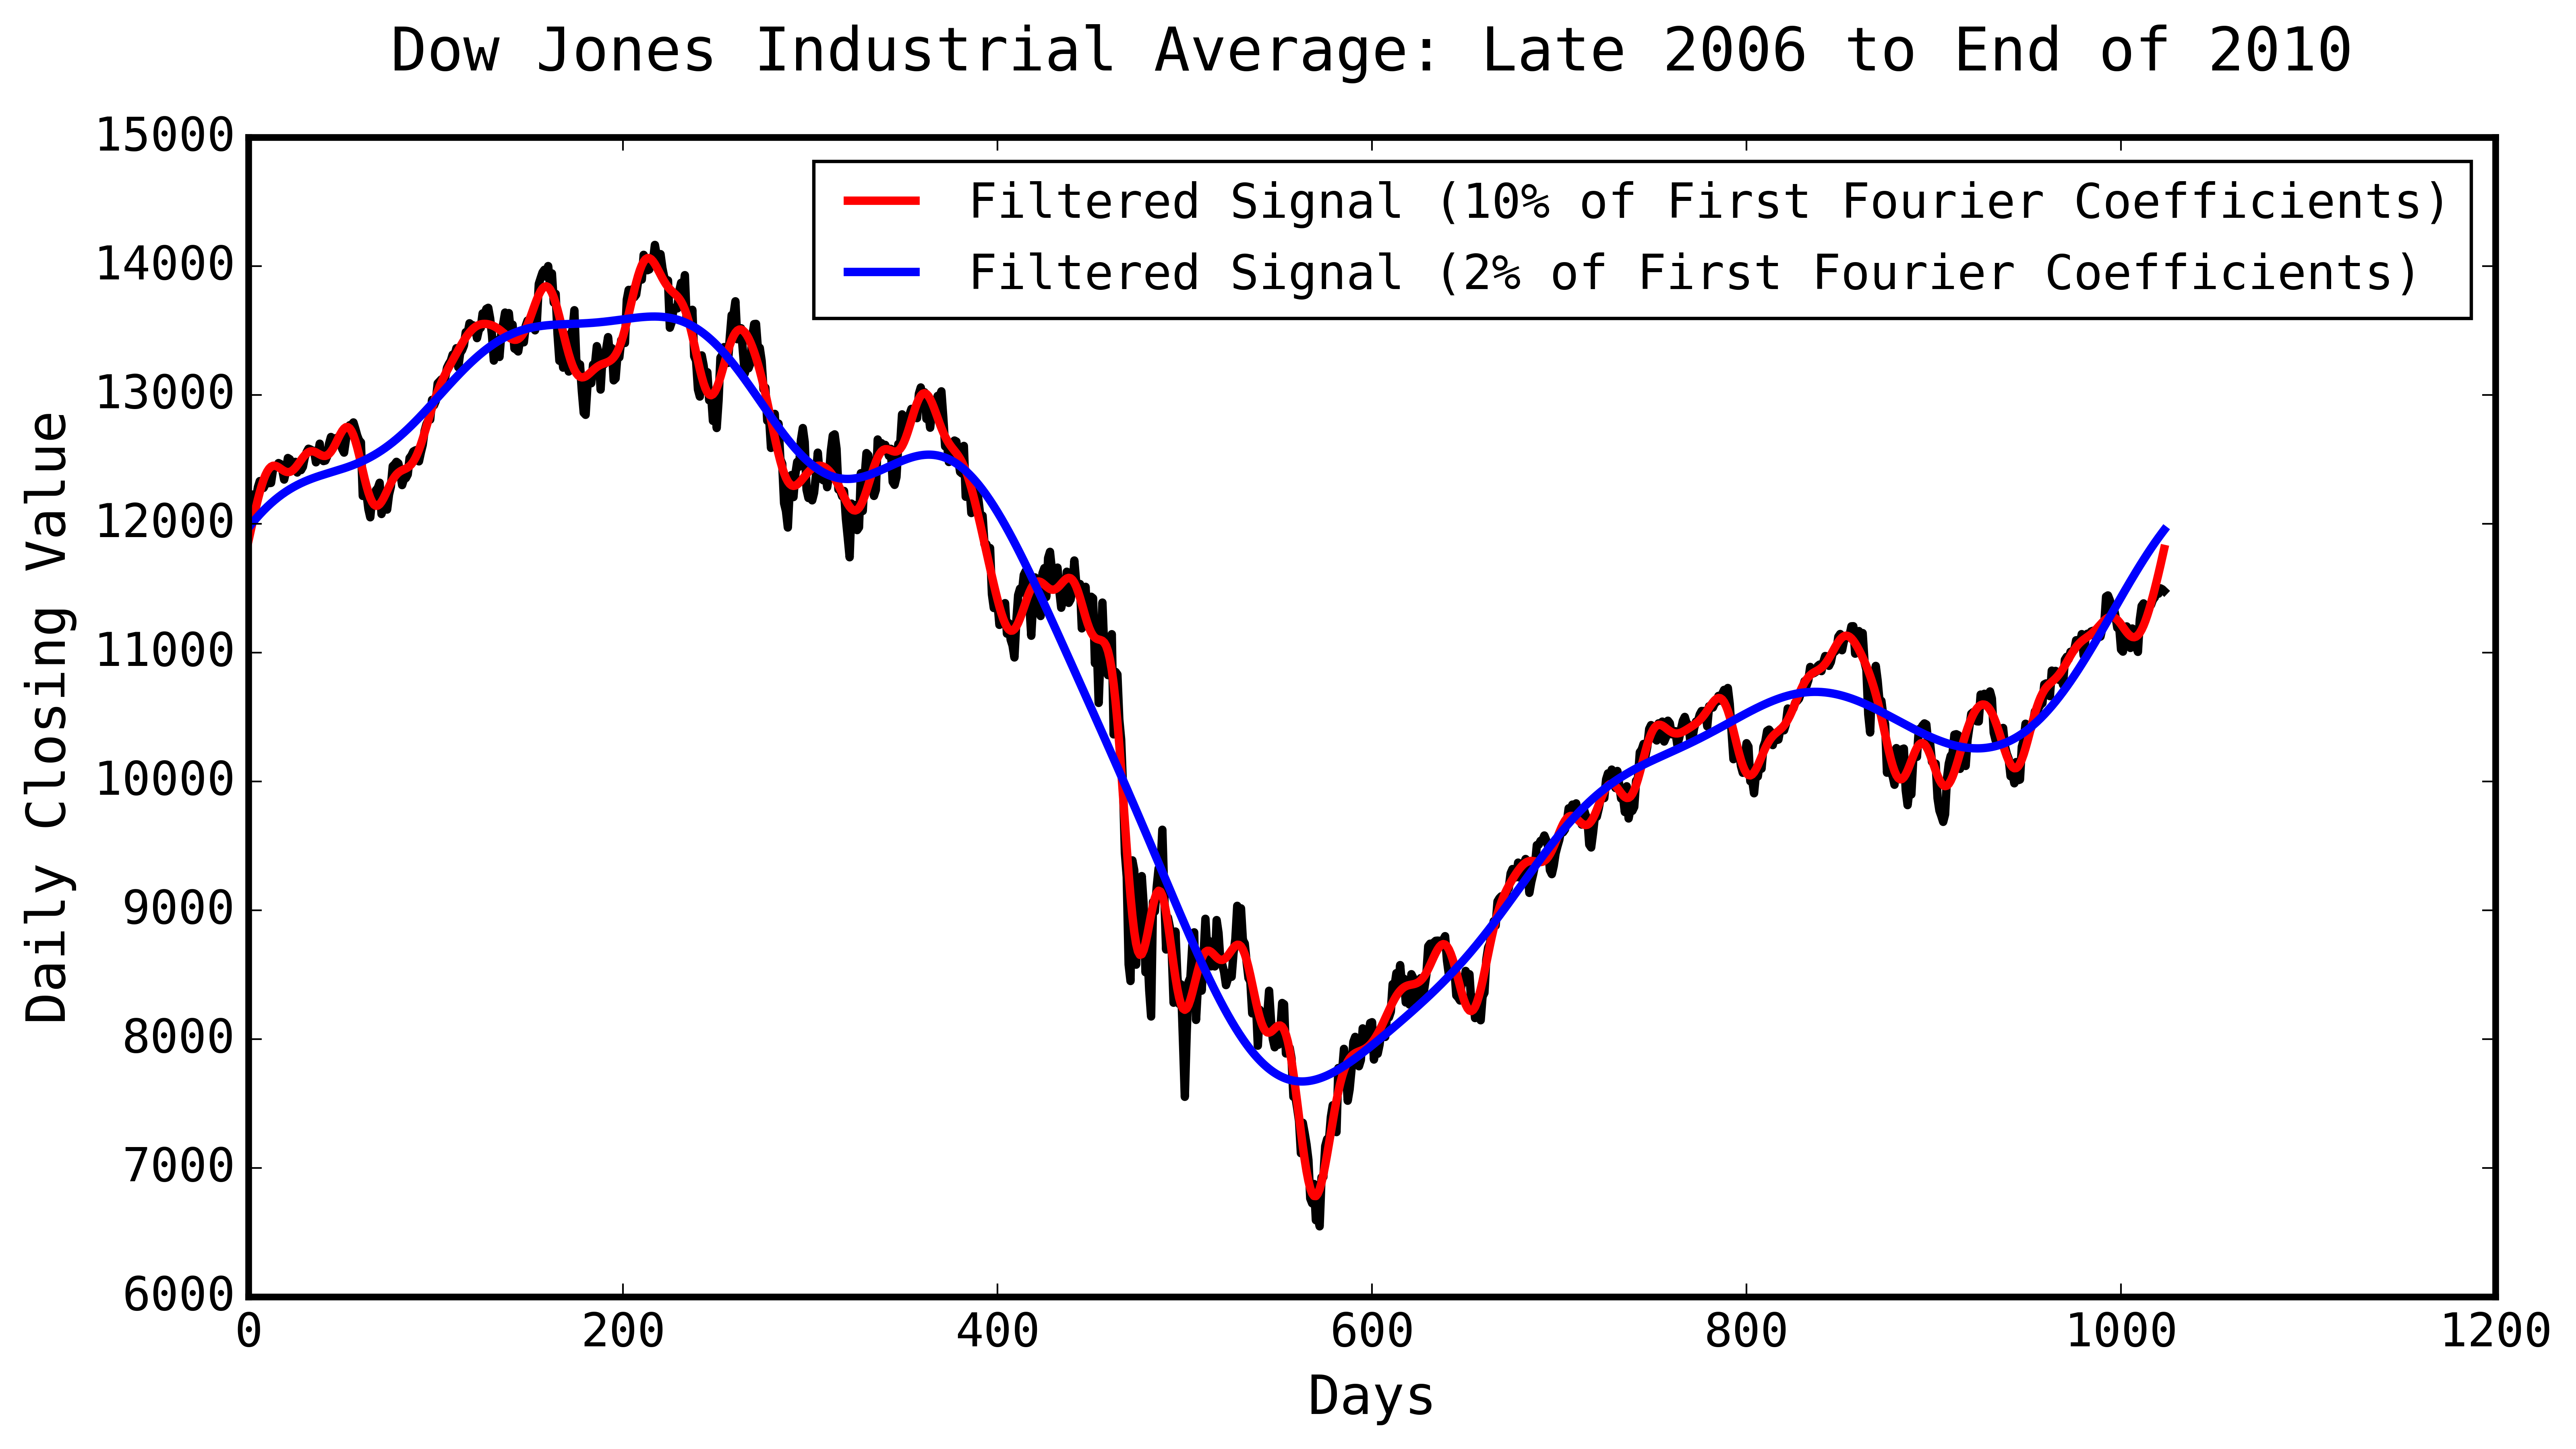
\includegraphics[width=0.95\textwidth]{figures/dow.png}
    \caption{Original Dow Jones data alongside reconstructions made by retaining the lowest $10\%$ (red) and $2\%$ (blue) of the Fourier coefficients.}
    \label{fig:dow-filtering}
\end{figure}

\subsection*{Exercise 7.9: Image Deconvolution}

The input image in \cref{fig:blurred-image} is quite blurry because each point in the original image has been spread over neighboring pixels by a point spread function. 

\begin{figure}[H]
    \centering
    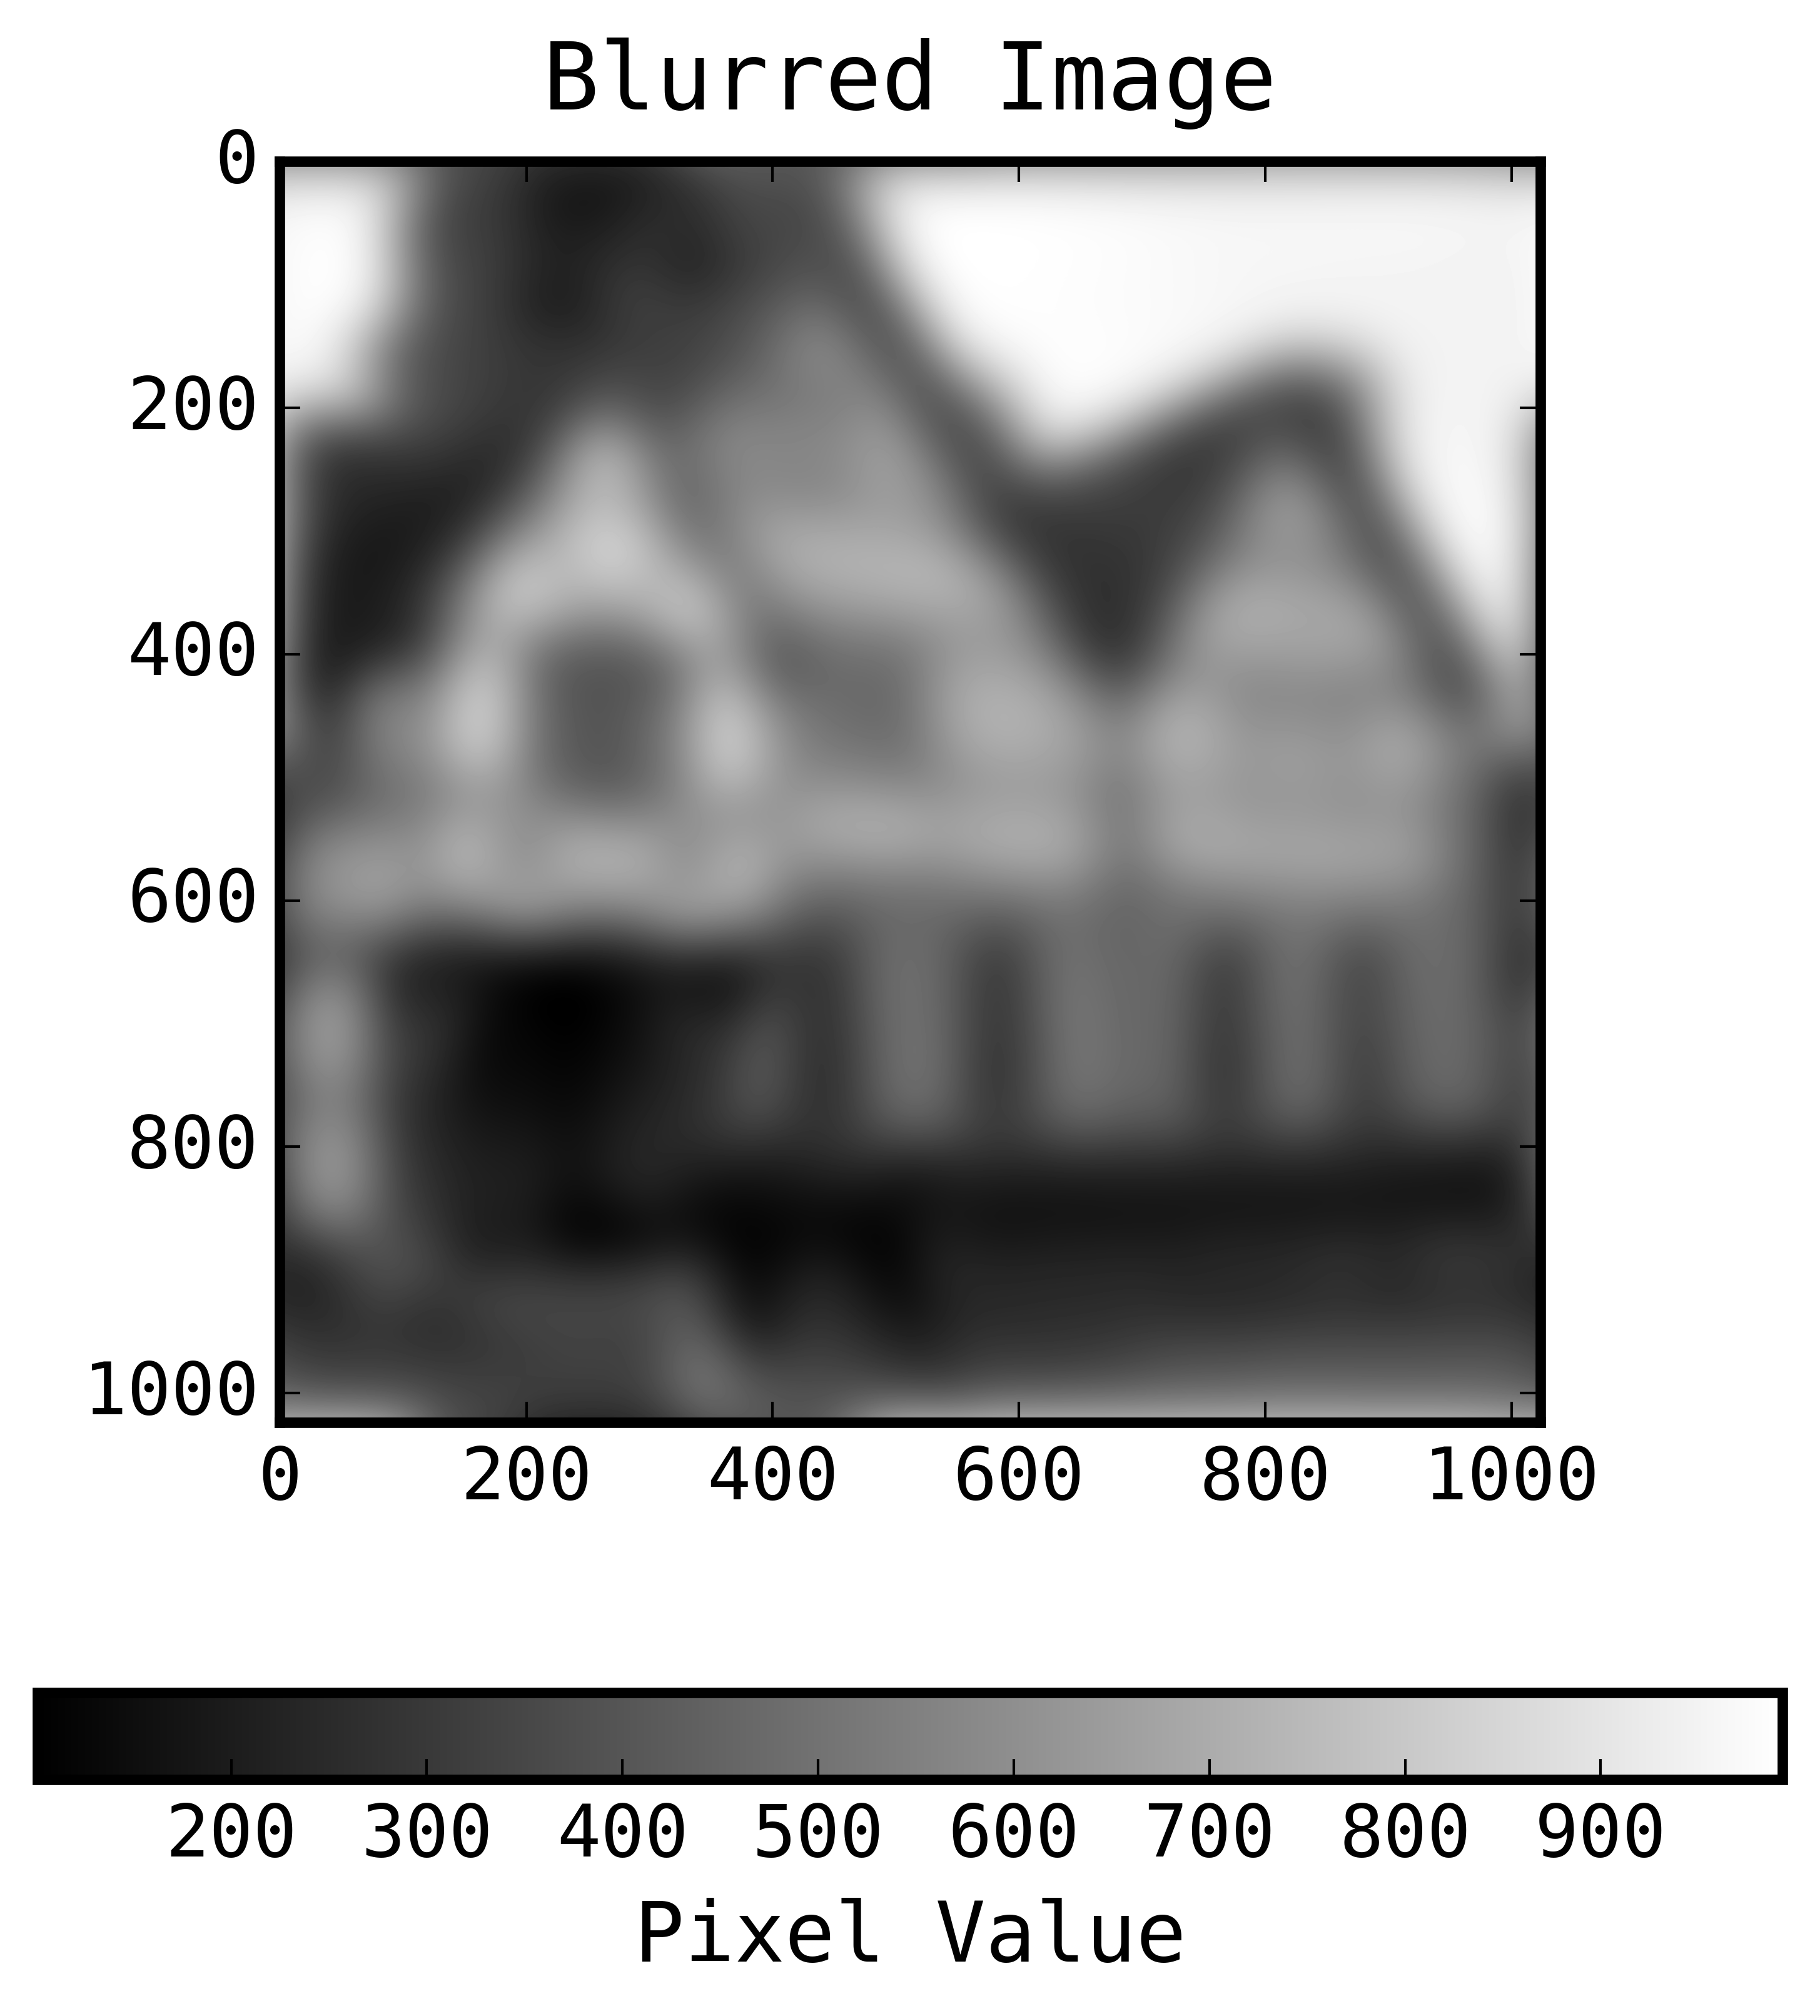
\includegraphics[width=0.7\textwidth]{figures/blur.png}
    \caption{The blurred input image.}
    \label{fig:blurred-image}
\end{figure}

The point spread function in \cref{fig:point-spread} was modeled as a periodic Gaussian with $\sigma=25$. Because the Gaussian is centered at the origin, its values wrap around the boundaries of the array, producing bright regions in all four corners.

\begin{figure}[H]
    \centering
    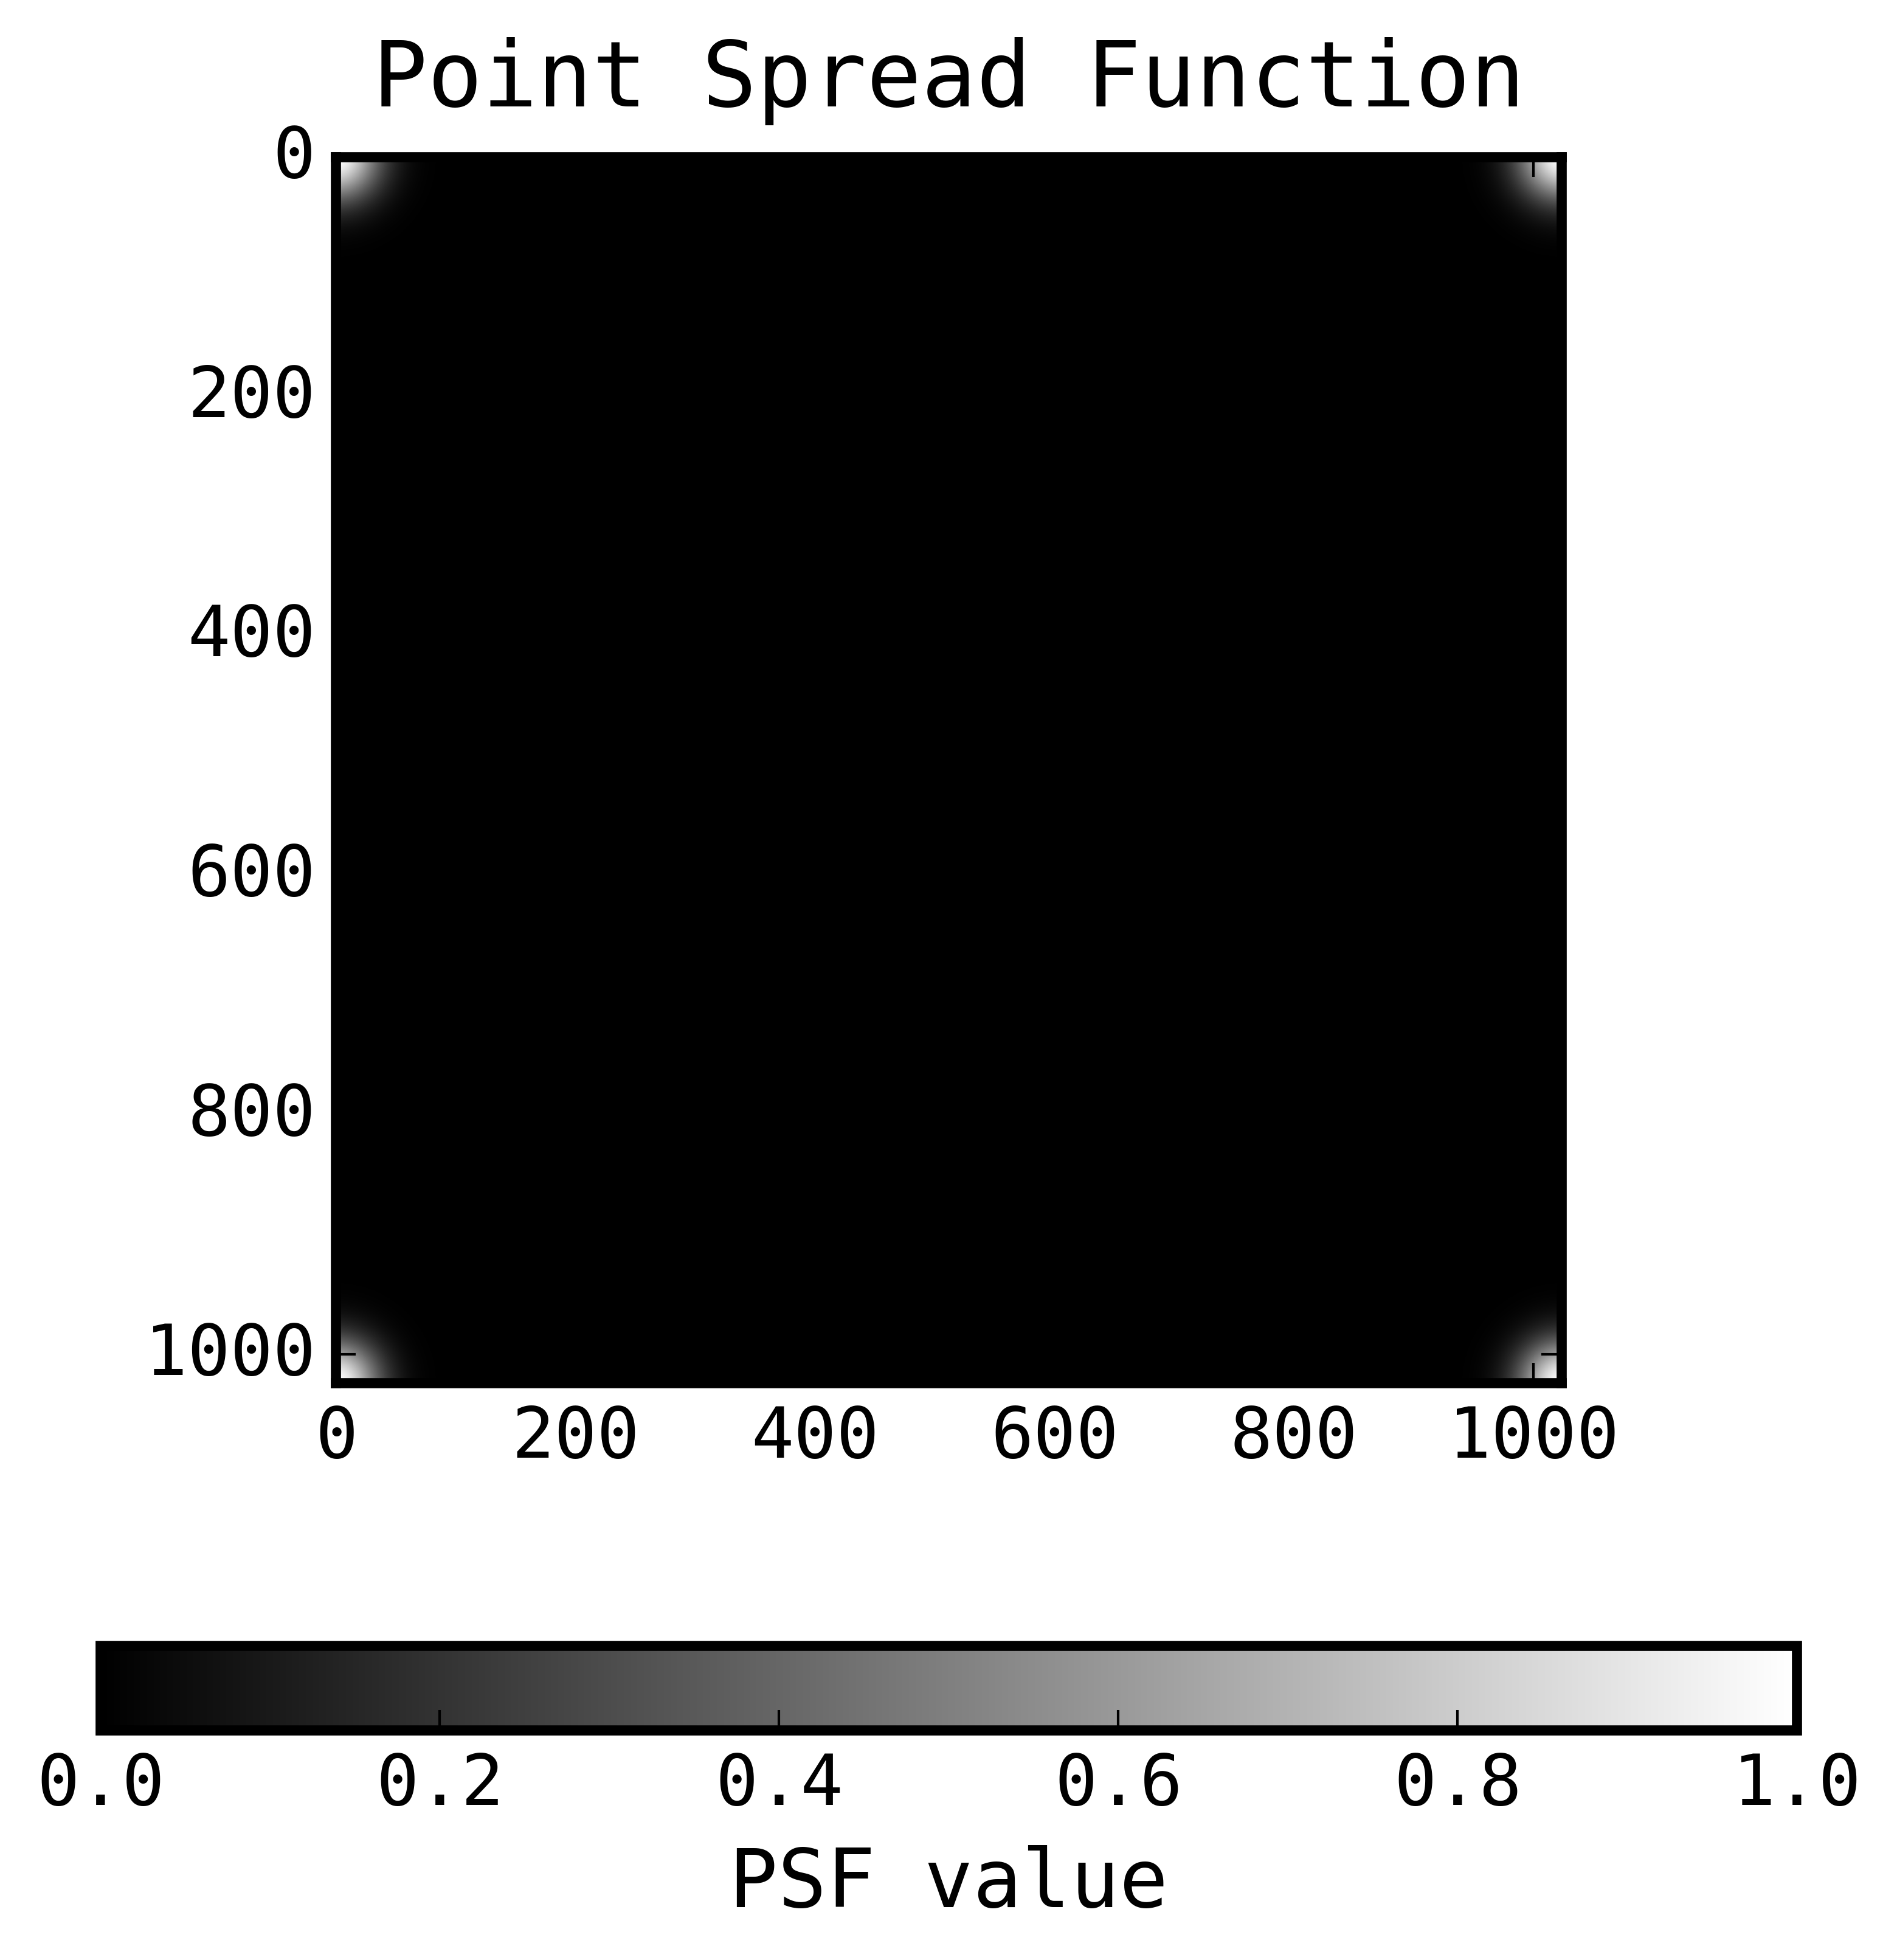
\includegraphics[width=0.7\textwidth]{figures/point_spread.png}
    \caption{Periodic Gaussian point spread function used to model the
    blurring.}
    \label{fig:point-spread}
\end{figure}

The blurred image and point spread function were transformed into Fourier space. Their Fourier coefficients were divided to reverse the convolution, except where the magnitude of the point spread function coefficient was less than $10^{-3}$. In those cases, the coefficient was left unchanged to avoid division by zero or by a very small number.

\begin{figure}[H]
    \centering
    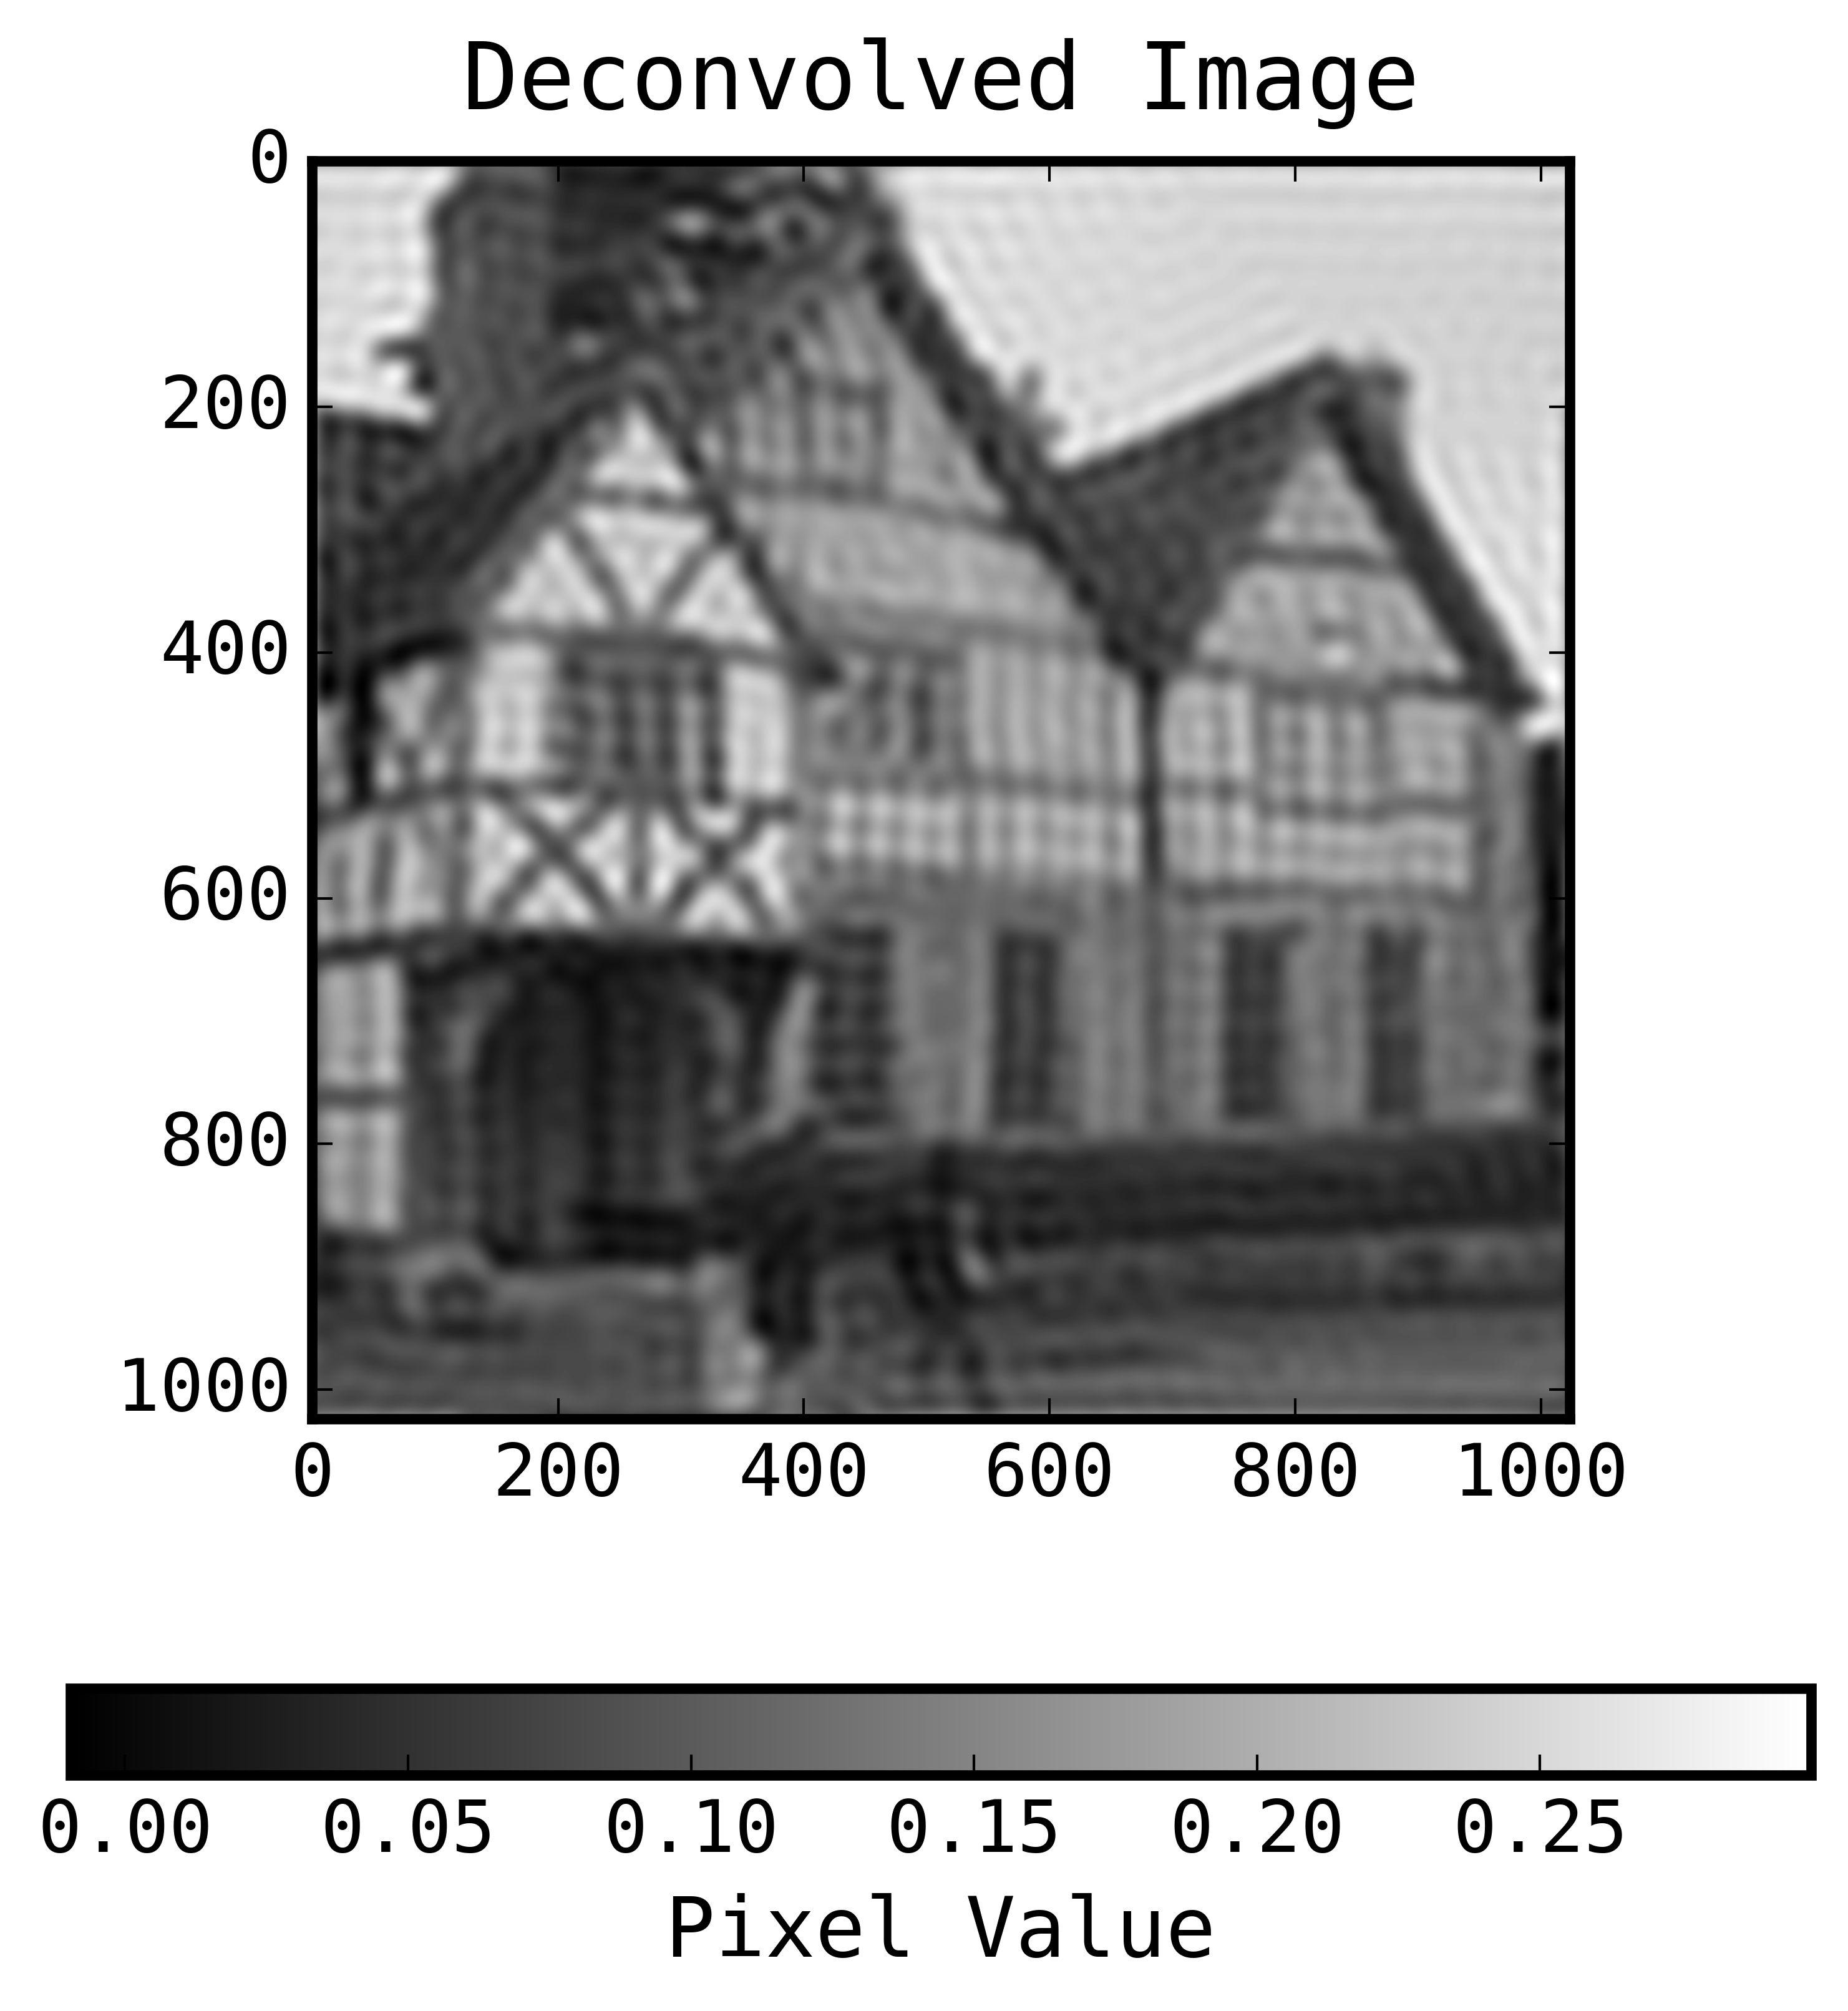
\includegraphics[width=0.7\textwidth]{figures/deconvolved.png}
    \caption{The image reconstructed by Fourier-space deconvolution.}
    \label{fig:deconvolved-image}
\end{figure}

The deconvolved image as seen in \cref{fig:deconvolved-image} is sharper than the original blurred image, and the main features become more distinguishable, such as the people in front of the house that were previously indistinct. However, the image is not perfectly restored because Fourier components that are strongly suppressed by the point spread function cannot be recovered in a reliable way, which means there is inevitably some loss in detail as each Fourier coefficient corresponds to a specific spatial frequency of detail. The threshold applied during the division prevents numerical instability but also means that some information remains blurred.

\section*{Code}

The link to the github repository for this homework assignment can be accessed by clicking \href{https://github.com/jpalmagomez/computational_physics_homework.git}{here}.

\clearpage

\end{document}